% \chapter{Result Tables}
% 
% 
\chapter{Trade Analysis Tables} \label{appendix:trade-tables}

\begin{figure}[b!]
    \begin{center}
        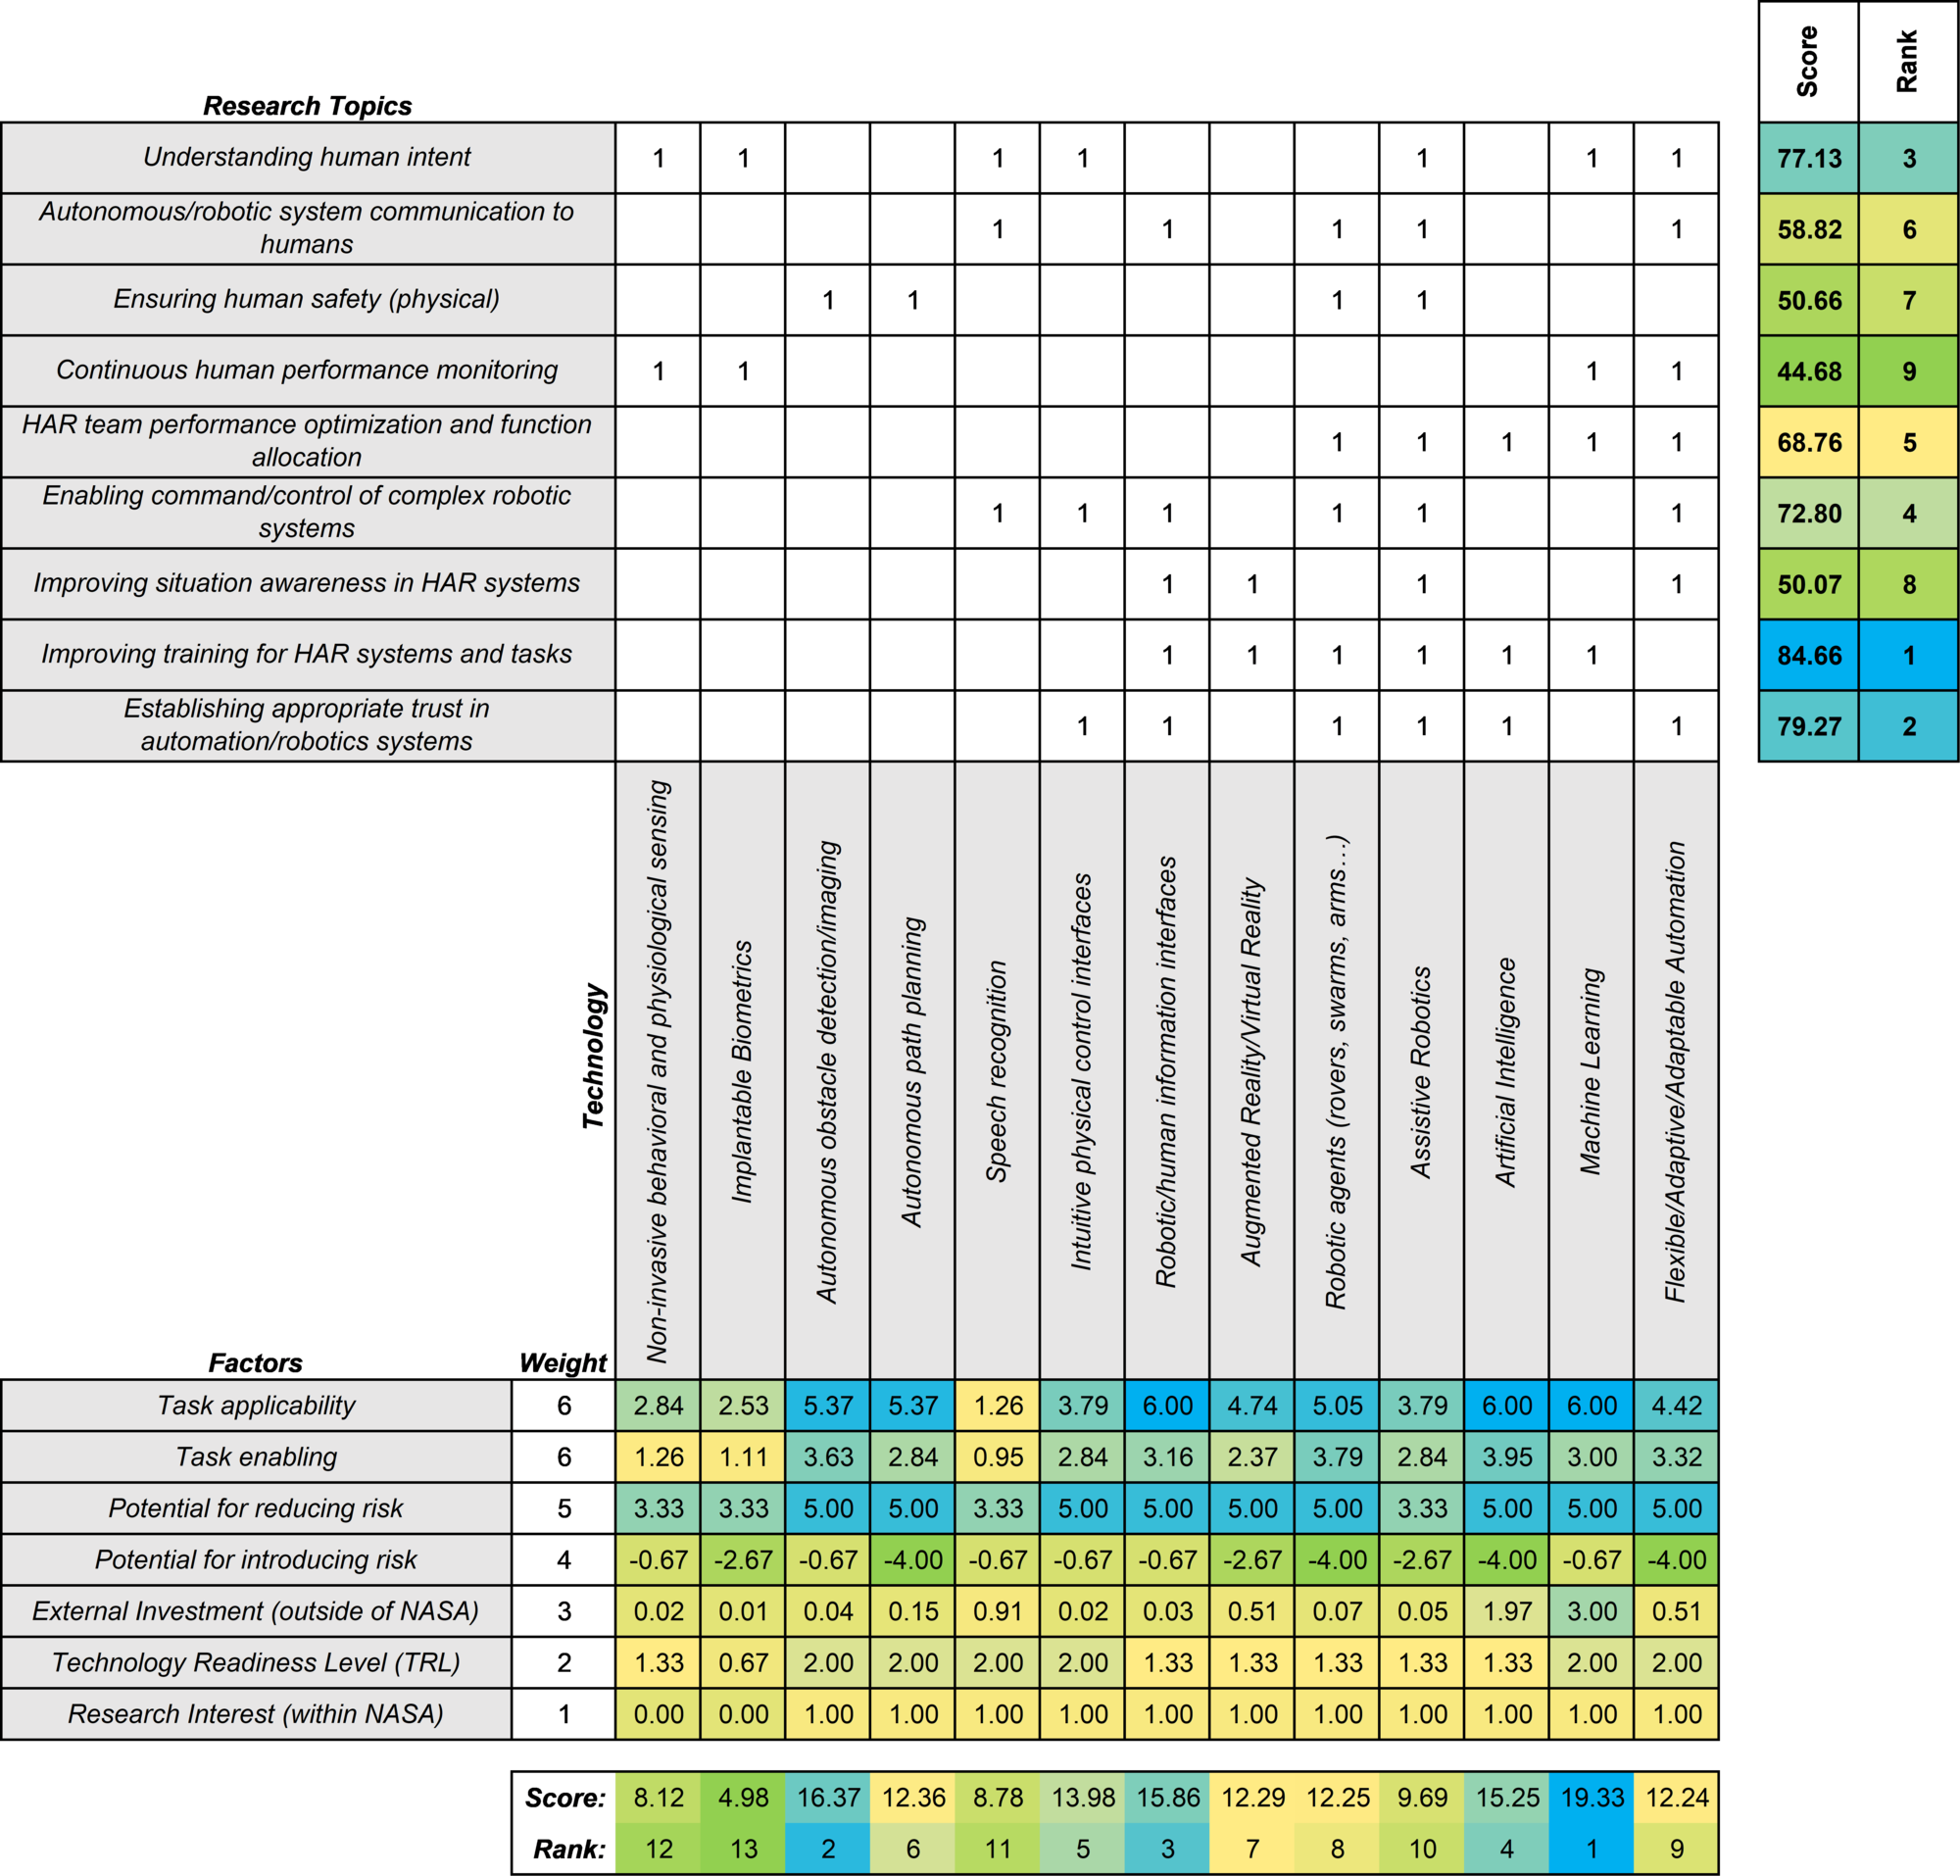
\includegraphics[width=0.8\linewidth]{figures/TradeStudy/figurea1.png}
        \caption{Top-level trade table with final research topic scores (top right), final technology scores based on factors (bottom) and weighted factor-level scores for each technology}
        % \label{figure:}
    \end{center}
\end{figure}

\begin{figure}[b!]
    \begin{center}
        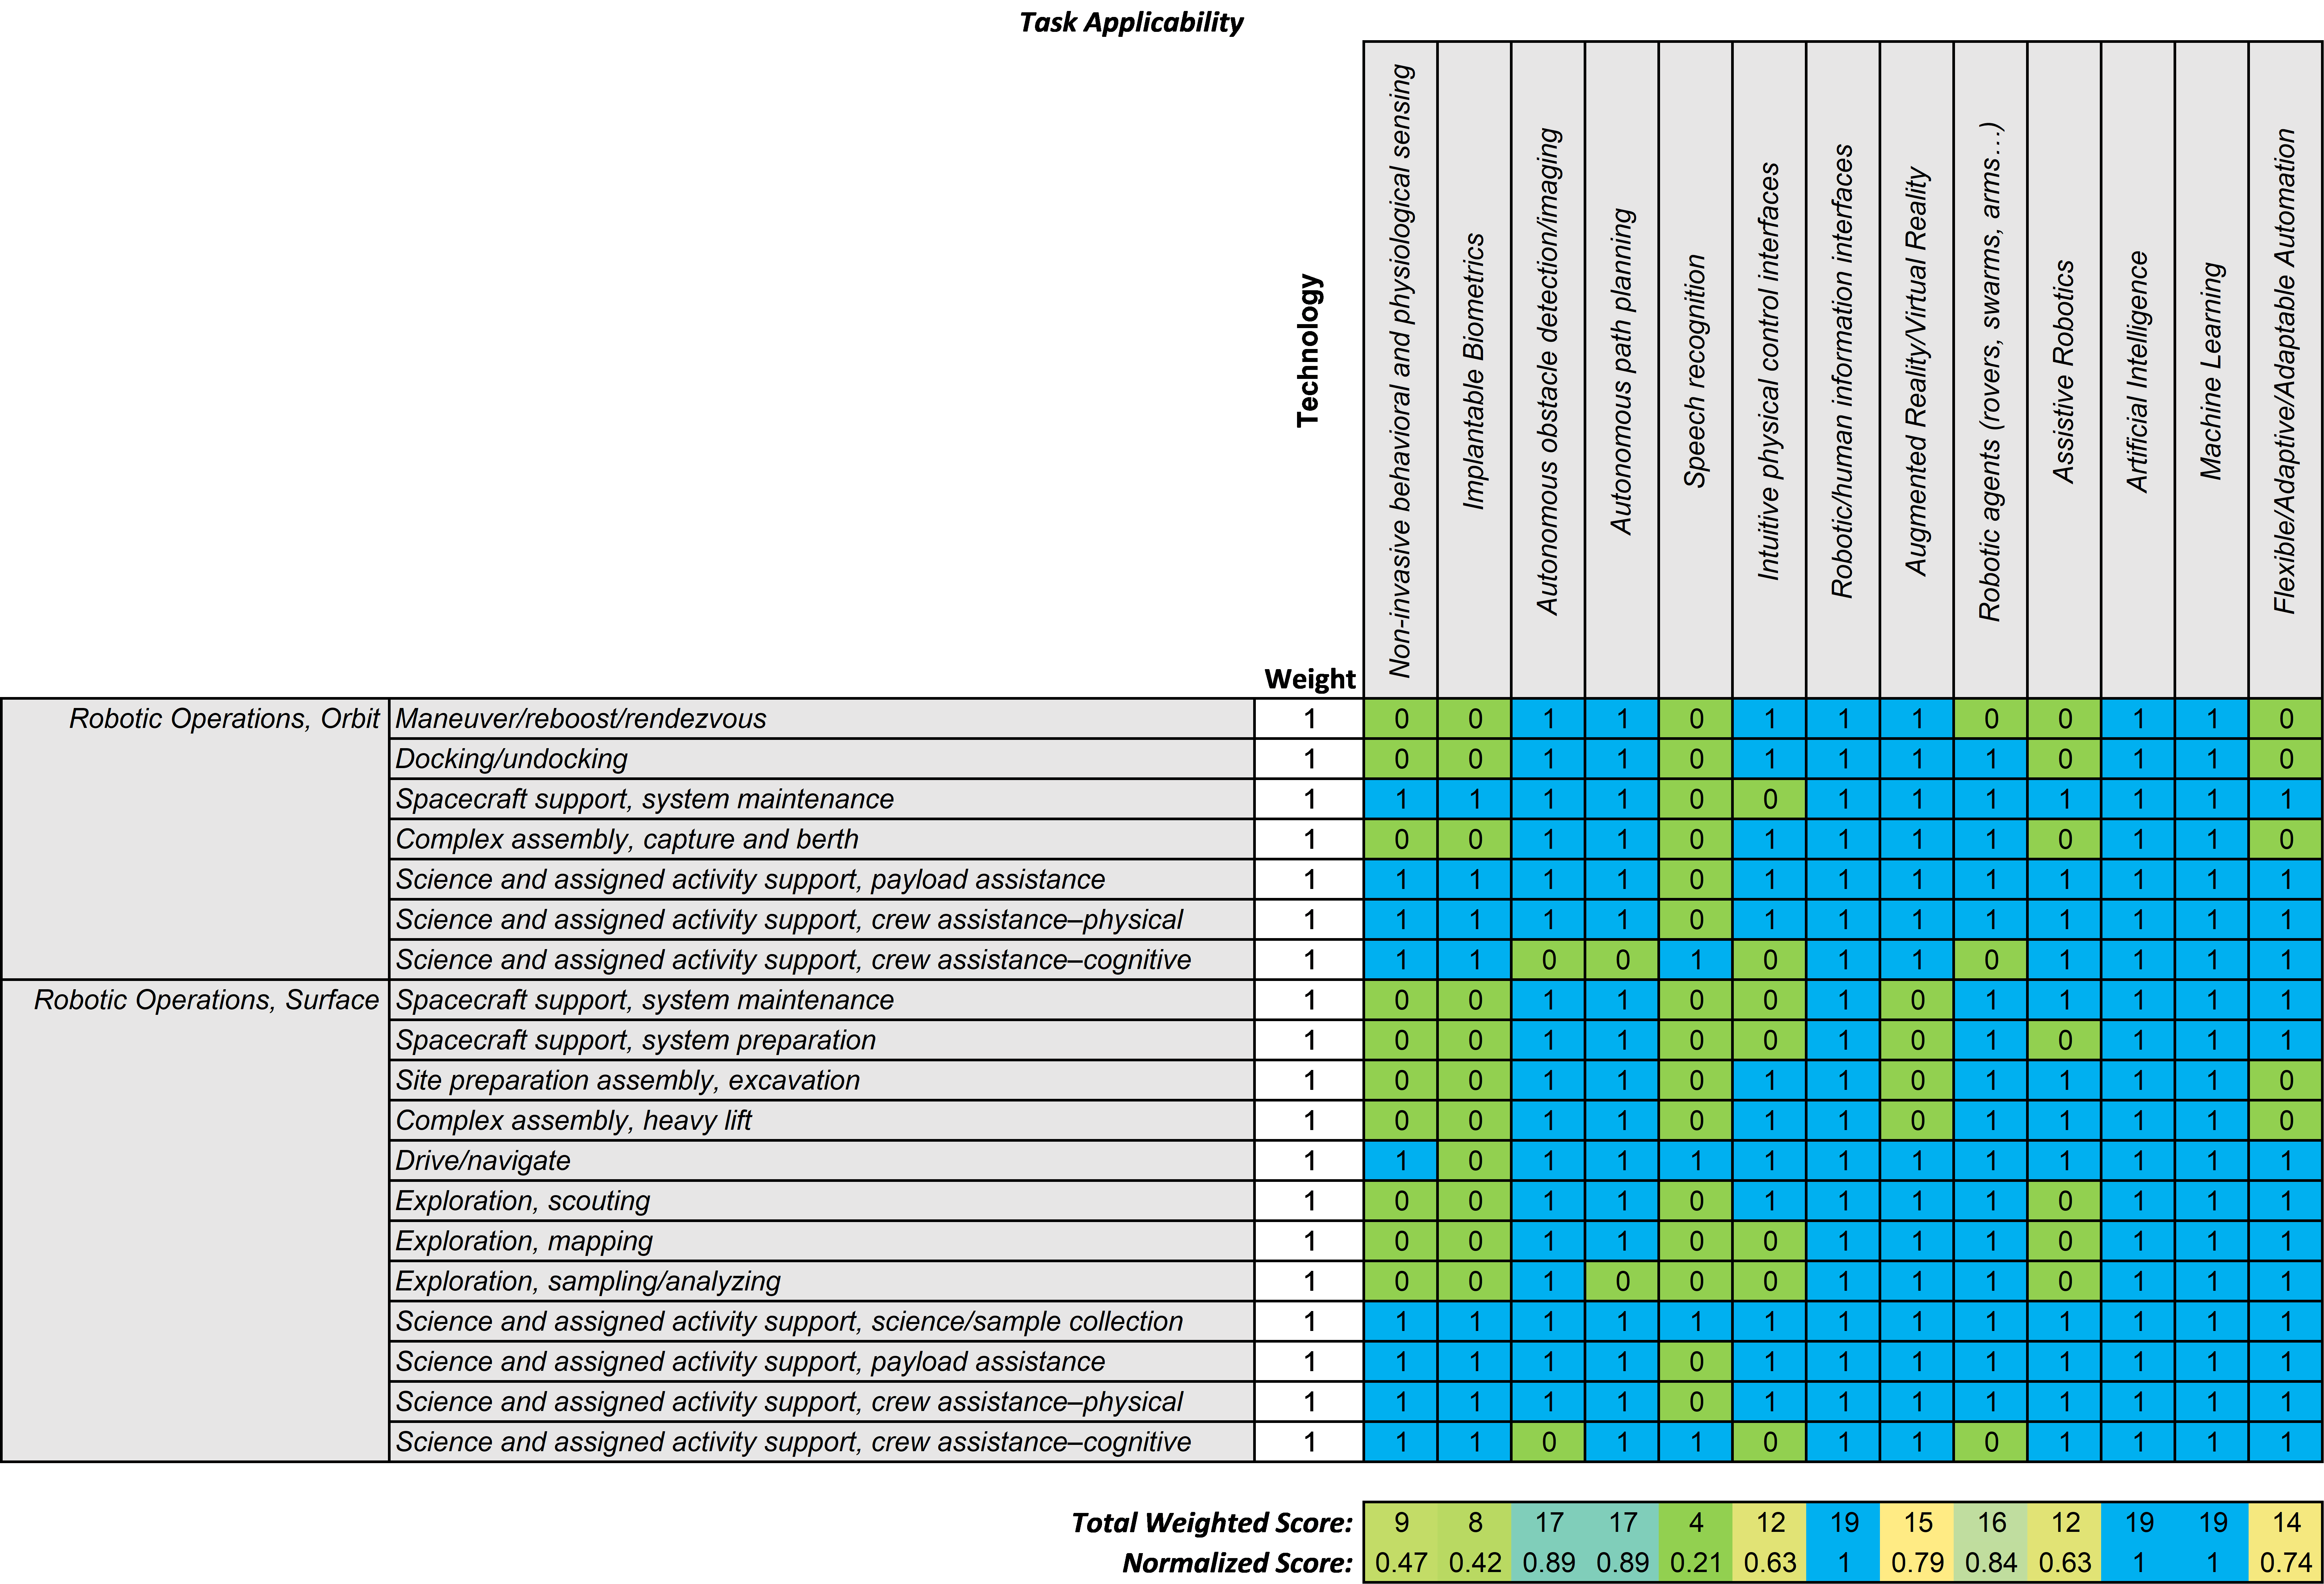
\includegraphics[width=0.8\linewidth]{figures/TradeStudy/figurea2.png}
        \caption{Technology to Task Applicability factor-level trade table}
        % \label{figure:}
    \end{center}
\end{figure}

\begin{figure}[b!]
    \begin{center}
        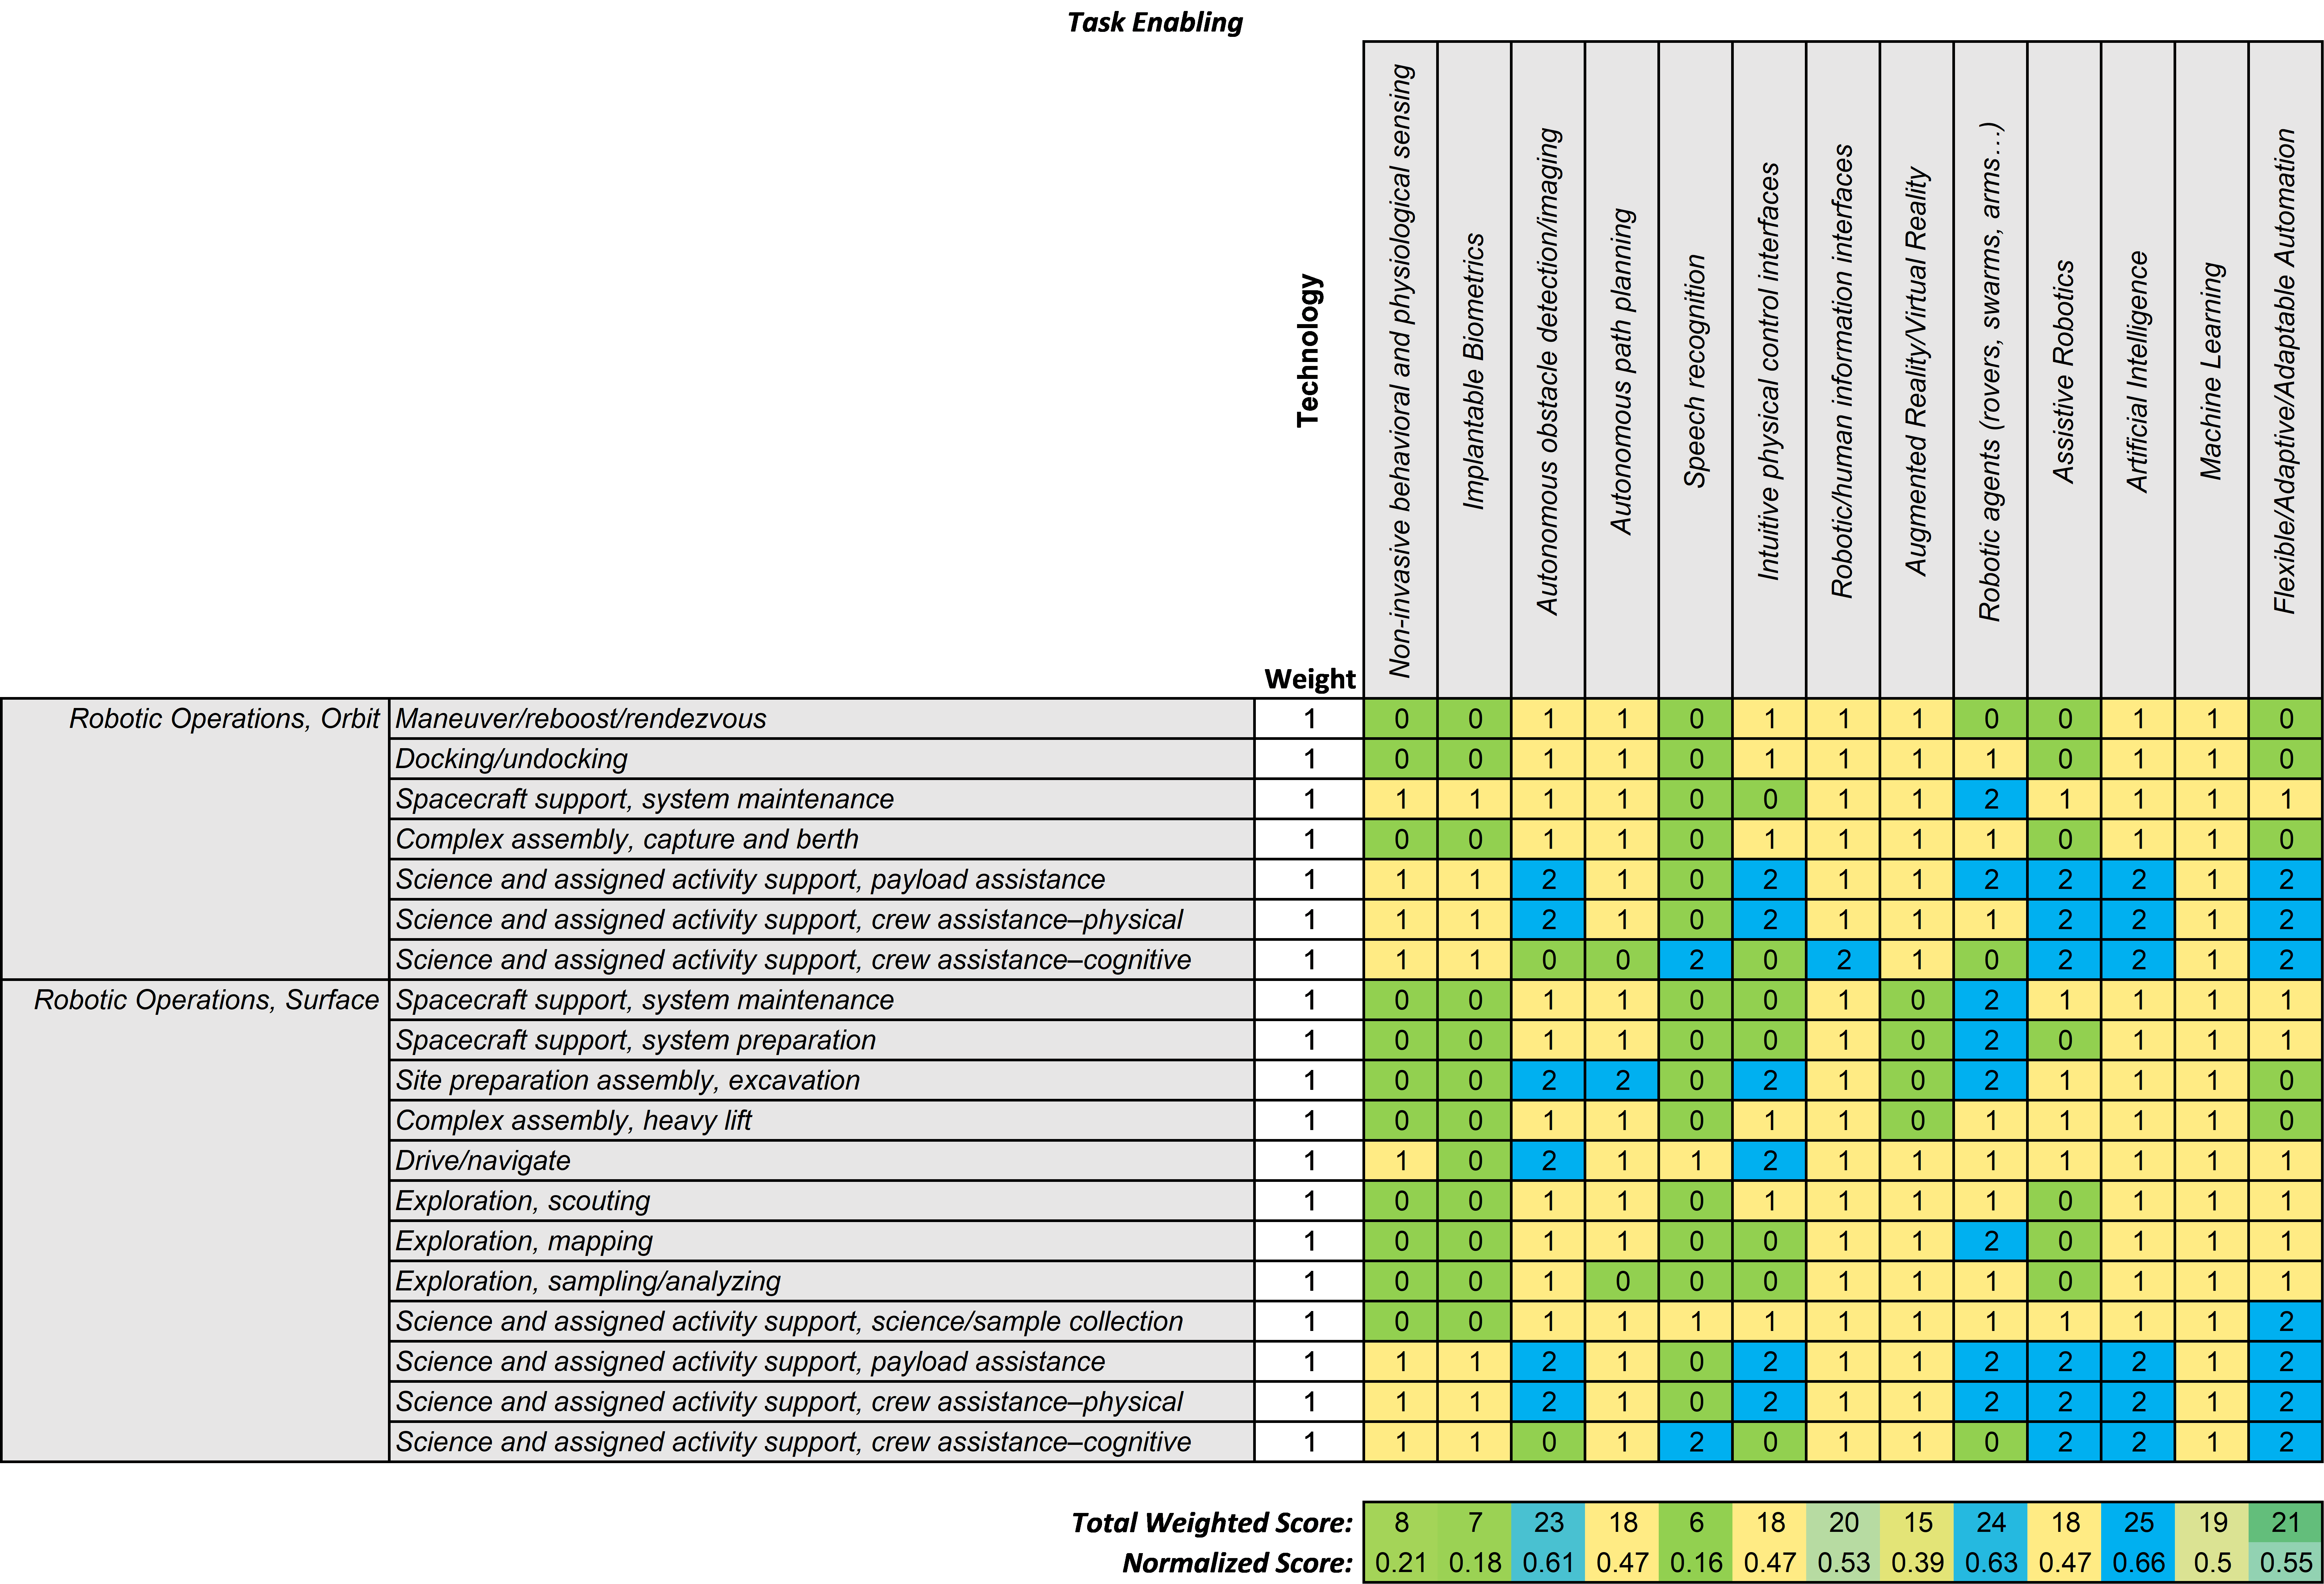
\includegraphics[width=0.8\linewidth]{figures/TradeStudy/figurea3.png}
        \caption{Technology to Task Enabling factor-level trade table}
        % \label{figure:}
    \end{center}
\end{figure}

\begin{figure}[b!]
    \begin{center}
        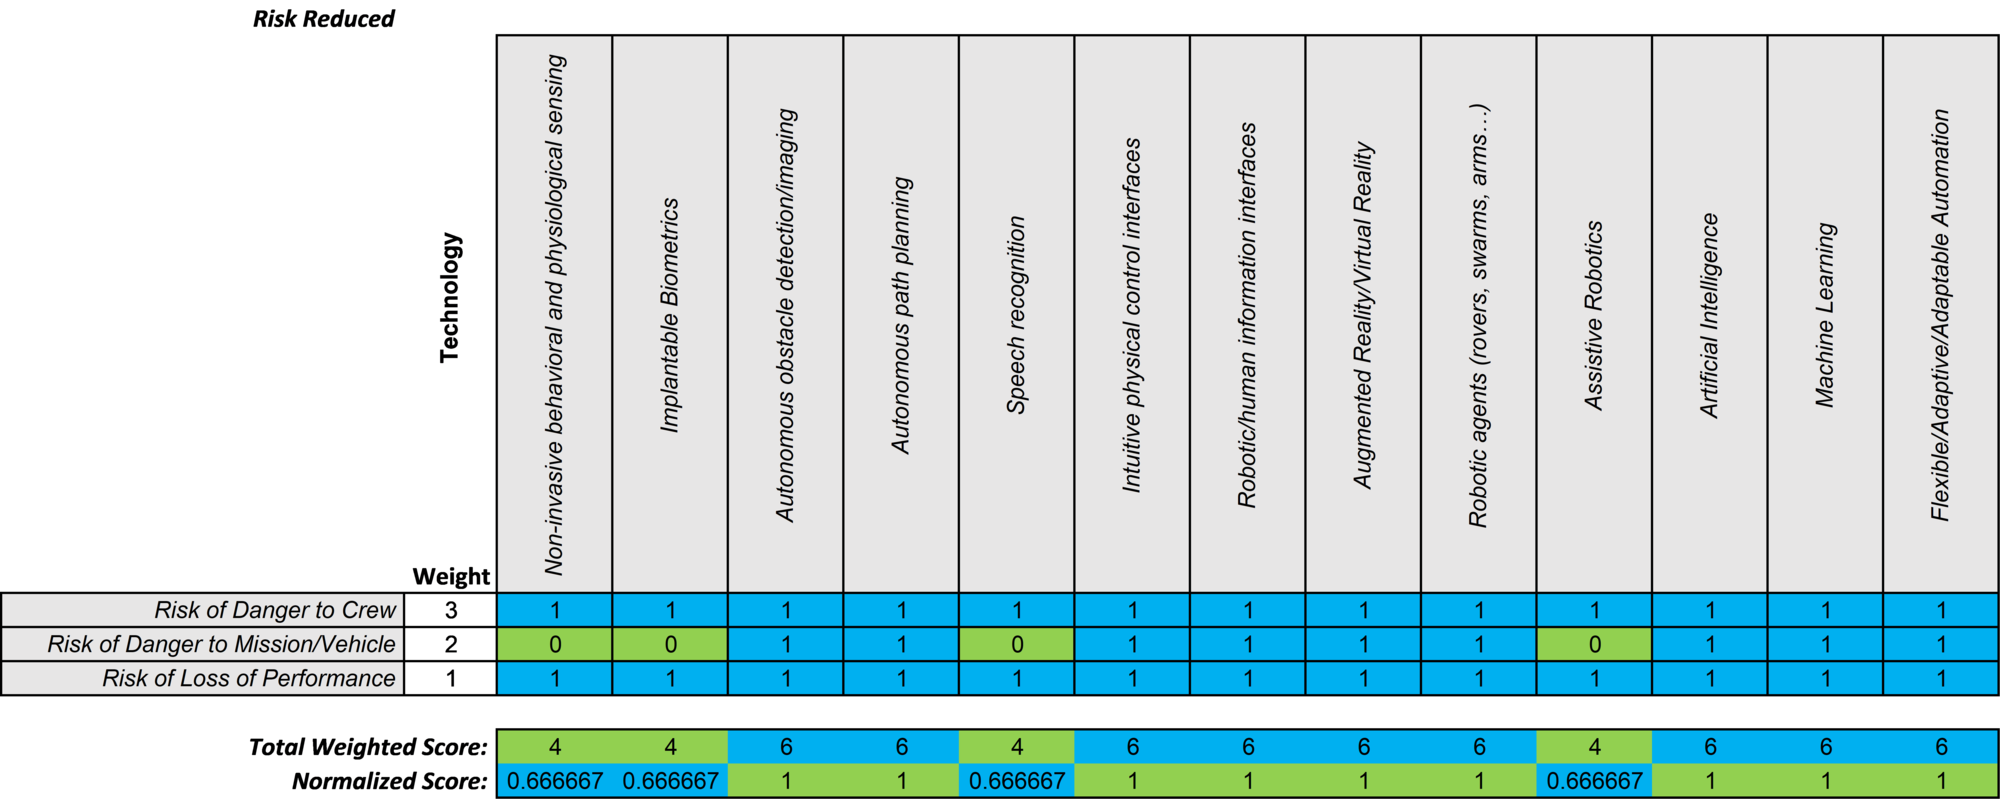
\includegraphics[width=0.8\linewidth]{figures/TradeStudy/figurea4.png}
        \caption{Technology to Risk Reduced factor-level trade table}
        % \label{figure:}
    \end{center}
\end{figure}

\begin{figure}[b!]
    \begin{center}
        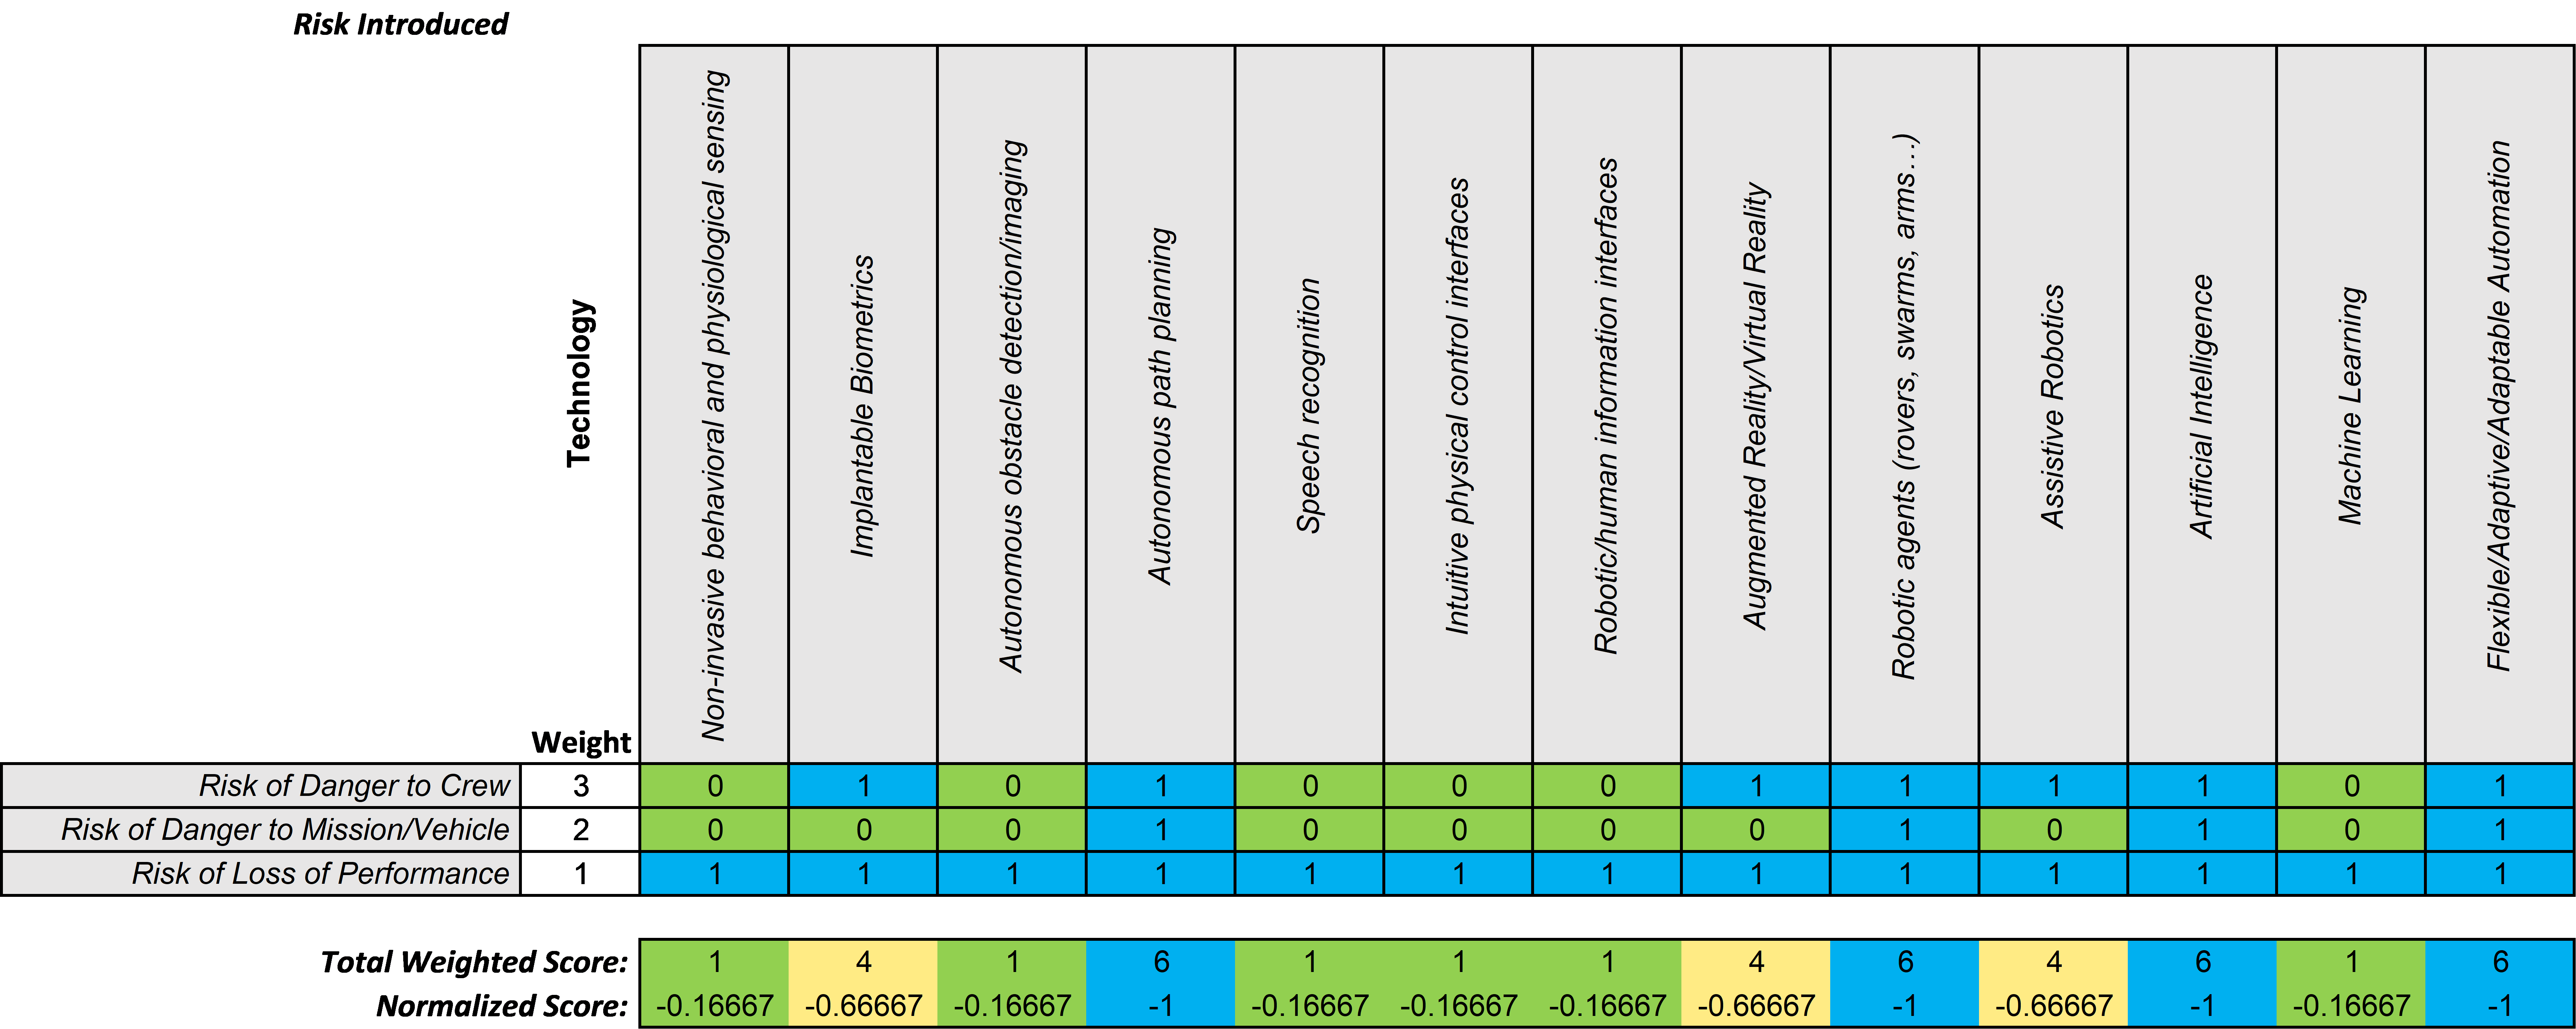
\includegraphics[width=0.8\linewidth]{figures/TradeStudy/figurea5.png}
        \caption{Technology to Risk Introduced factor-level trade table}
        % \label{figure:}
    \end{center}
\end{figure}

\begin{figure}[b!]
    \begin{center}
        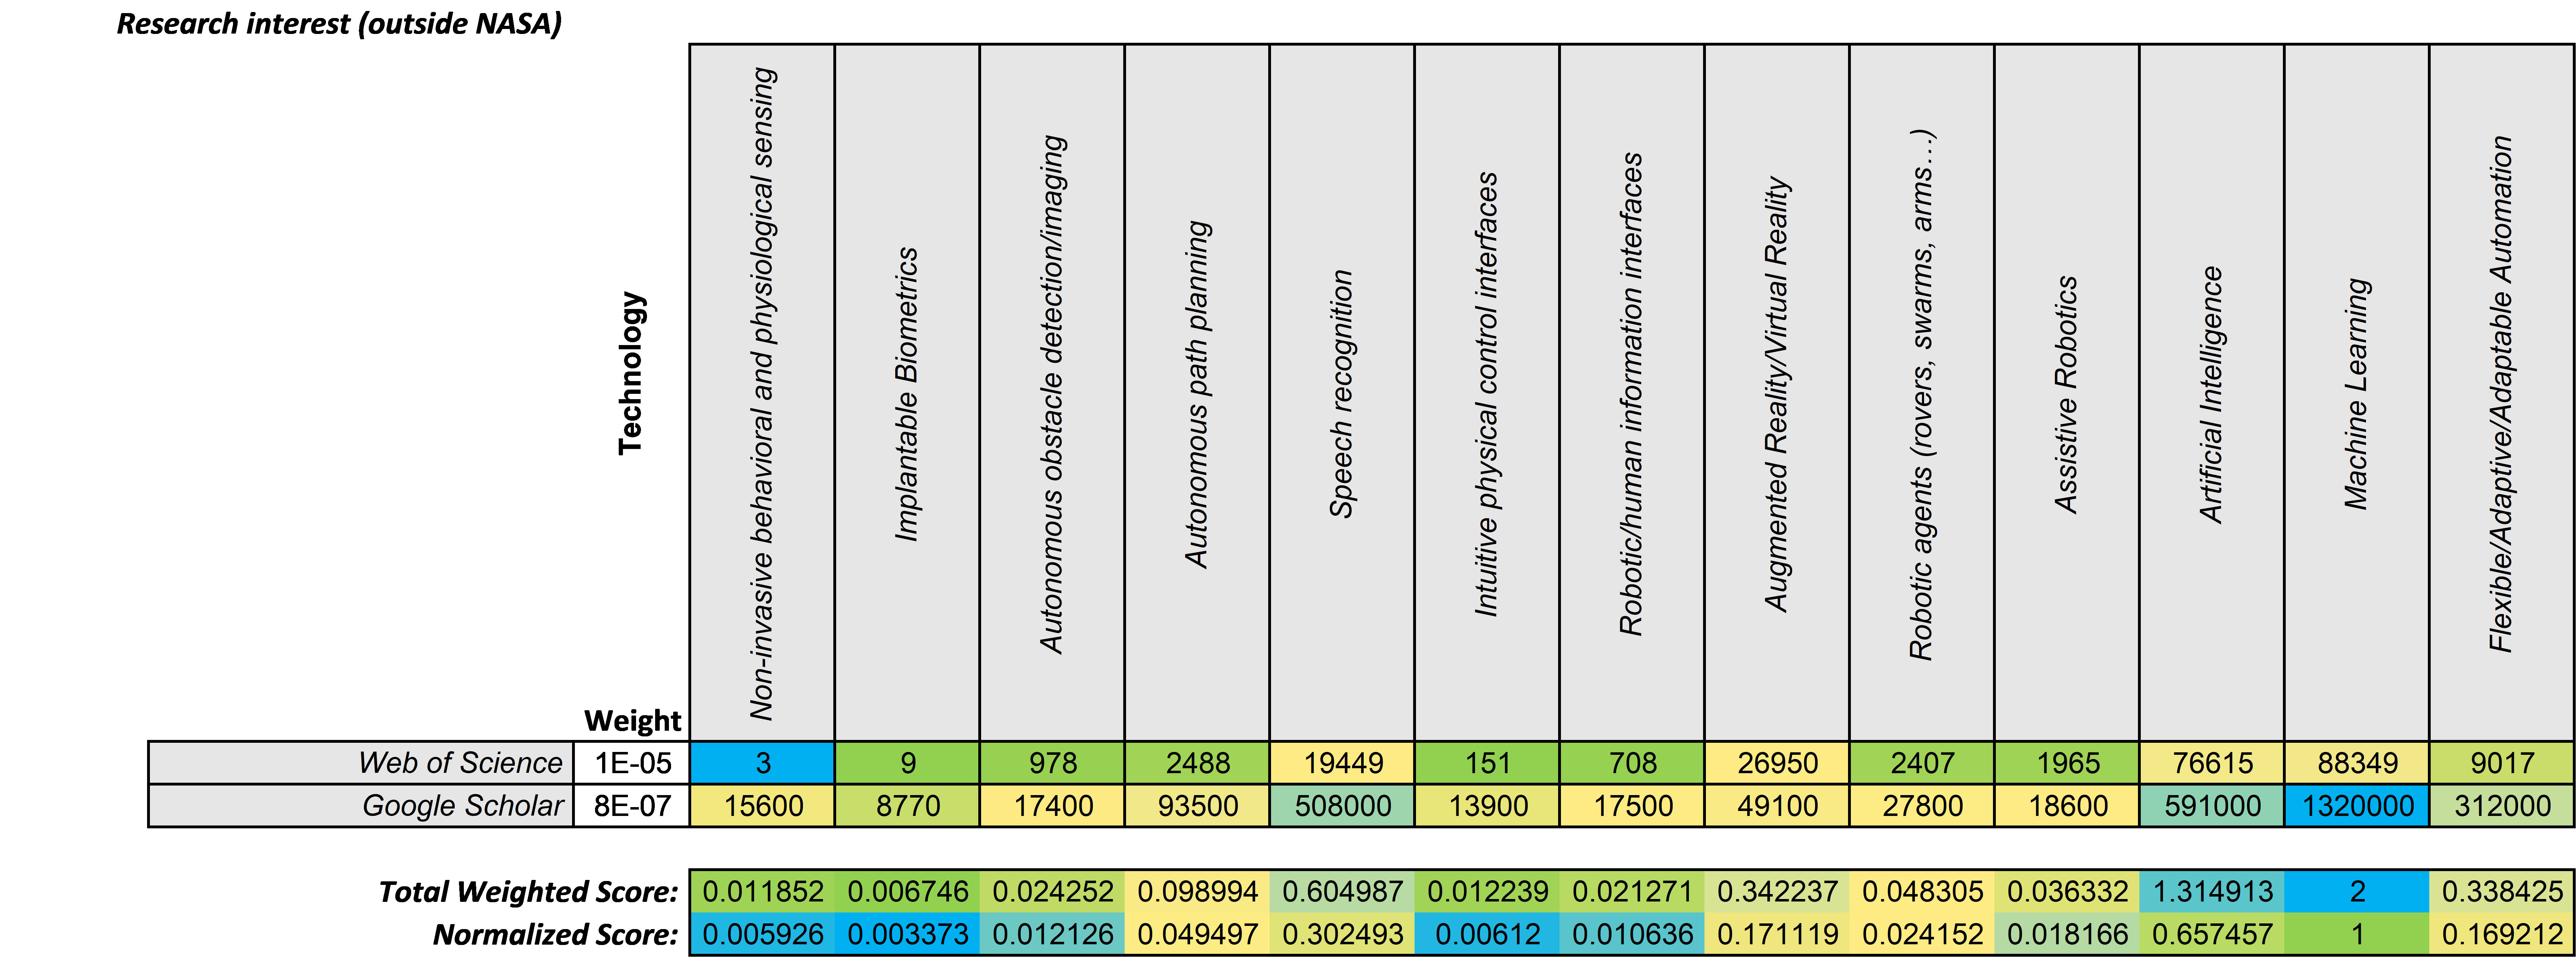
\includegraphics[width=0.8\linewidth]{figures/TradeStudy/figurea6.png}
        \caption{Technology to Research Interest (outside NASA) factor-level trade table}
        % \label{figure:}
    \end{center}
\end{figure}

\begin{figure}[b!]
    \begin{center}
        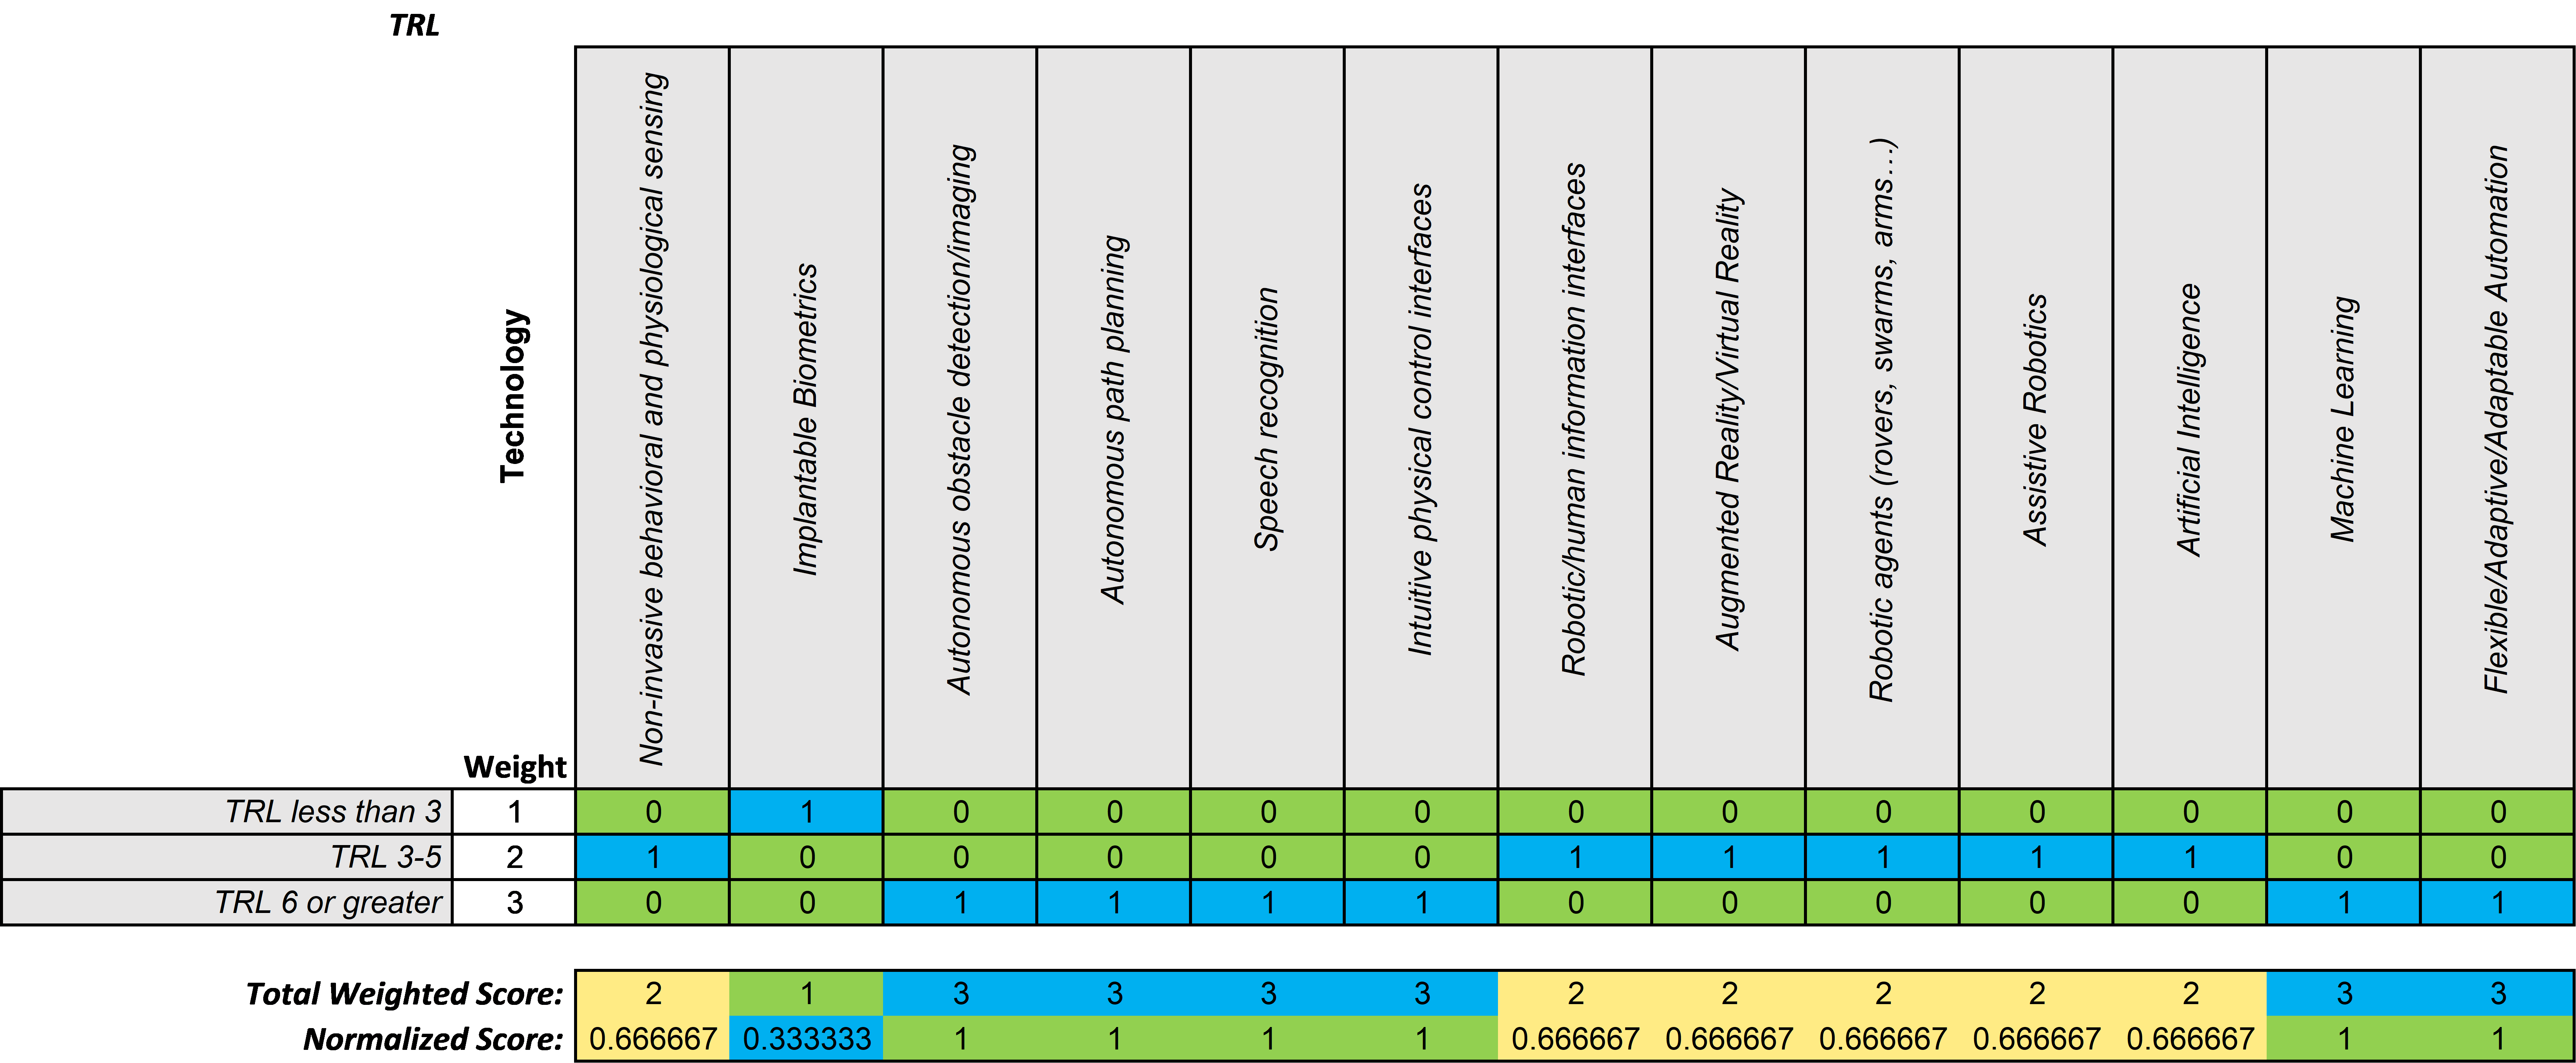
\includegraphics[width=0.8\linewidth]{figures/TradeStudy/figurea7.png}
        \caption{Technology to TRL factor-level trade table}
        % \label{figure:}
    \end{center}
\end{figure}

\begin{figure}[b!]
    \begin{center}
        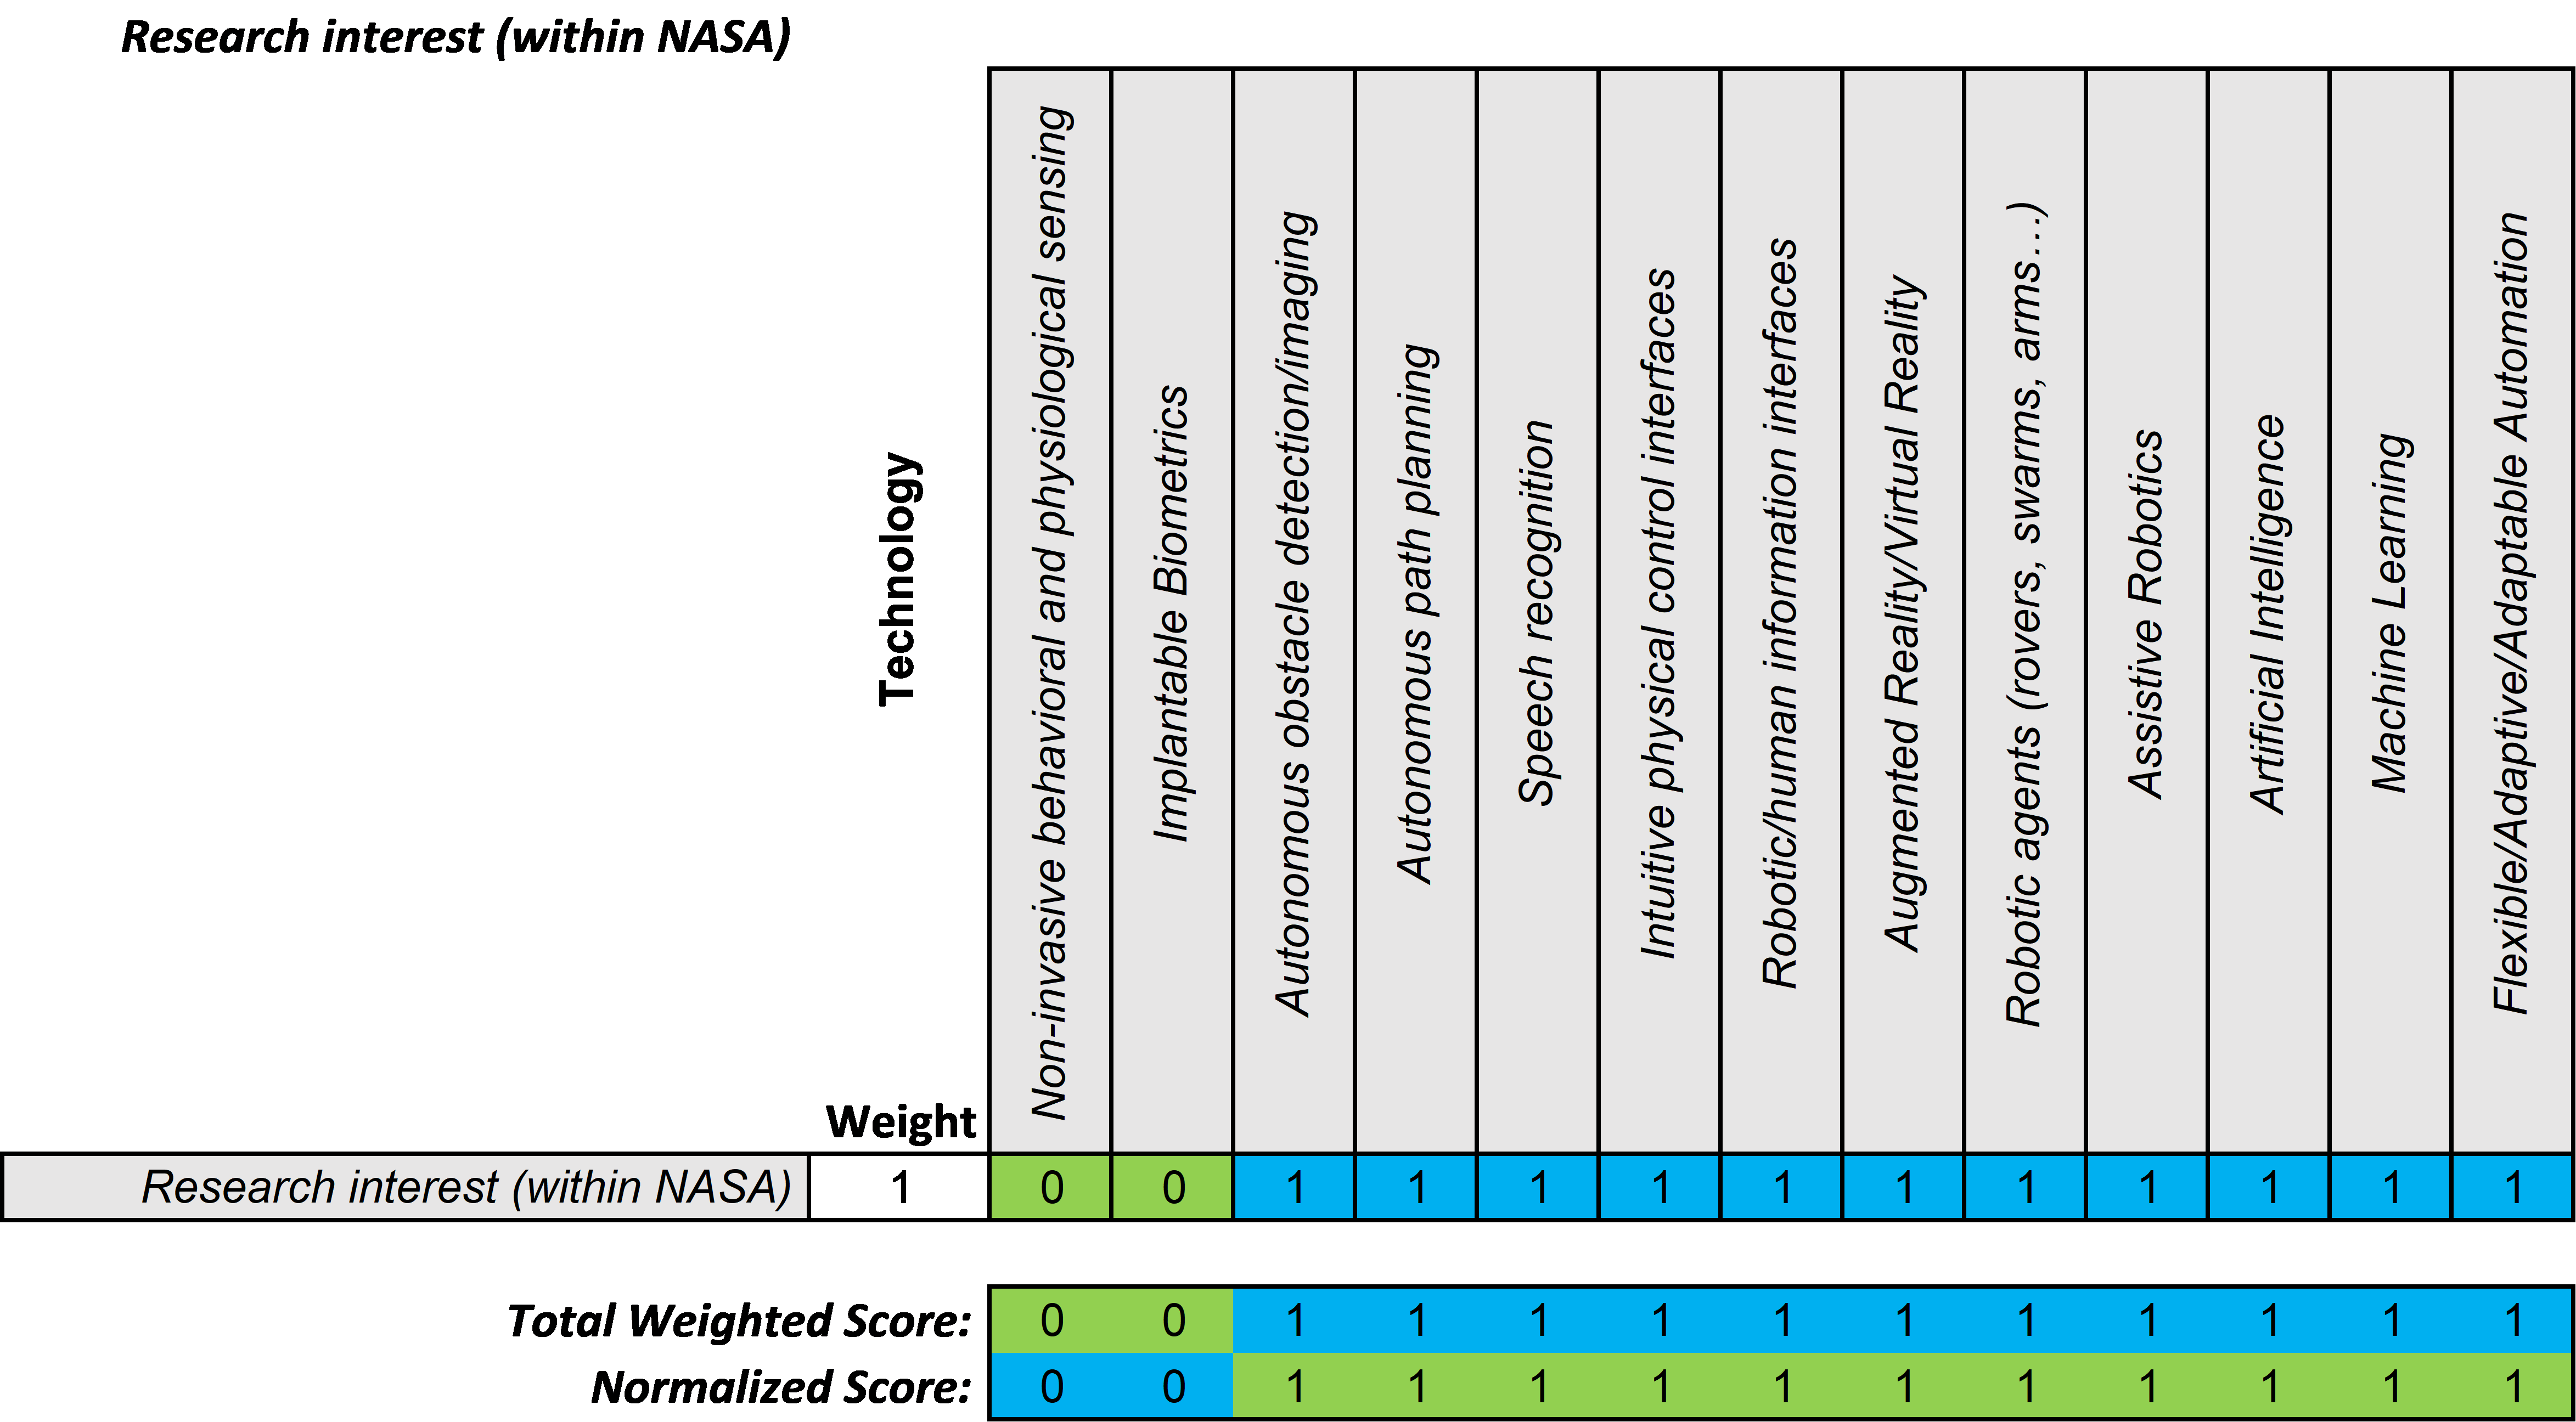
\includegraphics[width=0.8\linewidth]{figures/TradeStudy/figurea8.png}
        \caption{Technology to Research Interest (within NASA) factor-level trade table}
        % \label{figure:}
    \end{center}
\end{figure}

% Appendix B: Subject Matter Expert Summary of Backgrounds
% The SMEs interviewed to gather background information on the HARI trade space all have extensive experience in either HAR integration research, human factors, or both, in their respective fields. Additionally, three SMEs have experience in related fields: one person in data analytics, and two others in psychology/neuroscience. The SMEs have a wide range of experience addressing different research applications, captured in Table B1.

% SME	Background	Expertise
% 		Space	Aviation	Military	Medical	Automotive	Locomotive	Robotics (general)
% 1	Industry		x	x
% 2	Industry		x	x
% 3	Academia	x	x			x	x	x
% 4	Industry,
% Former NASA	x	x		x
% 5	Military			x	x			x
% 6	Academia, Industry				x	x
% 7	Academia	x	x	x			x
% 8	Academia,
% Industry		x					x
% 9	Academia	x			x			x
% 10	Industry,
% Former NASA	x			x	x
% Table B1: Background and application area expertise of interviewed subject matter experts

% Appendix C: Annotated Bibliography
% Parasuraman, Raja, and Christopher D. Wickens. "Humans: Still vital after all these years of automation." Human factors 50.3 (2008): 511-520.
% 	In their 2008 review, Parasuraman and Wickens discuss major discoveries and developments in levels and stages of automation, reliance on and compliance with automation, and adaptive automation. "Parasuraman, Sheridan, and Wickens (2000) accordingly proposed an extension of the LOA concept to four information-processing stages: (a) information acquisition, (b) information analysis, (c) decision making, and (d) action, with each stage having its own LOA scale (for similar scales, see Endsley & Kaber, 1999; Endsley & Kiris, 1995)."
% Ososky, Scott, et al. "Building Appropriate Trust in Human-Robot Teams." AAAI Spring Symposium: Trust and Autonomous Systems. 2013.
% 	In their 2013 paper, Ososky et al. describe autonomous, intelligent robots as teammates, rather than tools, and describe the importance of appropriate, rather than maximal, trust in the human-robot team. They discuss how human operators must create a sufficiently developed mental model of a robot to appropriately use it for tasks which the robot can perform superiorly to the human. They note that inaccurate mental models can create "pitfalls for robotic system misuse or disuse", and that accurate mental models are required for the human to appropriately trust the robot. They argue that appropriate trust in the robotic system leads to how the robotic system is ultimately used.
% Beer, Jenay M., Arthur D. Fisk, and Wendy A. Rogers. "Toward a framework for levels of robot autonomy in human-robot interaction." Journal of Human-Robot Interaction 3.2 (2014): 74-99.
% 	In their 2014 paper, Beer, Fisk, and Rogers outline a framework for levels of robot autonomy (LORA) for human-robot interaction (HRI), with the goal of allowing researchers to identify the impacts of autonomy on the interaction between human and robot. They outline a set of guidelines which can serve as "(1) a set of guidelines suggesting task and environmental influences on robot autonomy, (2) guidelines for determining or measuring autonomy, (3) a taxonomy for categorizing autonomy, and finally, (4) a set of HRI variables that may be influenced by robot autonomy."
% Chen, Jessie YC, and Michael J. Barnes. "Human–agent teaming for multirobot control: A review of human factors issues." IEEE Transactions on Human-Machine Systems 44.1 (2014): 13-29.
% 	In their 2014 paper, Chen and Barnes identified important human factors issued related to human-agent teams in multirobot control. They conclude that agents acting as interfaces between human operators and intelligent systems are an efficient way for operators to supervise multiple systems, while natural language processing is not required, the agents must have the ability to recognize operator intent, and that mixed initiative architectures can take advantage of both the human's expertise and the agent's precision and ability to act quickly. Mixed initiative systems, a subset of flexible automation, which allows for a dynamic level of automation based on the operator's state and events in the environment. Chen and Barnes further note the importance of transparency in effectively calibrating operator trust in an autonomous system.
% Kehoe, Ben, et al. "A survey of research on cloud robotics and automation." IEEE Trans. Automation Science and Engineering 12.2 (2015): 398-409.
% 	Kehoe et al.'s 2015 paper considers robots and automation systems that rely on externally networked support, and focuses on the benefits of the cloud, including: big data, cloud computing, collective robot learning, and human computation. They note the state of the art in each of these areas while considering the current challenges and future directions research must should be taken. New issues associated with the rise in cloud technology include the need for techniques to consider time varying latency and quality of service, privacy concerns, and big data cleaning and filtering techniques. The note three levels at which a cloud computing framework are currently established: Infrastructure as a Service (IaaS), where bare operating systems are available; Platform as a Service (PaaS), where more structure is provided, including access to application frameworks, databases, and programming languages; and Software as a Service (SaaS), where software is made available online rather than as a local service. They conclude by proposing a fourth cloud framework, Robotics and Automation as a Service (RAaaS), which merges PaaS and SaaS frameworks to provide a cloud service which processes inputs for robotics, suggests output actions, and monitors results to update future recommendations.
% Rautaray, Siddharth S., and Anupam Agrawal. "Vision based hand gesture recognition for human computer interaction: a survey." Artificial Intelligence Review 43.1 (2015): 1-54.
% 	Rautaray and Agrawal's 2015 survey provides a summary of progress in the field of vision-based hand gesture recognition and reviews the three main phases of hand gesture recognition: detection, tracking, and recognition. They analyze existing literature and note the required advances to further improve hand gesture recognition systems. They note the primary application domains of hand gesture recognition are desktop applications, followed by gaming and sign language. In terms of the challenges of operating in real-time and robustness, the authors find that comparisons are difficult as there is no commonly accepted baseline technique to compare to. Psychological aspects of gestures have been found to play an important role in hand gesture recognition systems. The authors find that, despite plenty of research into the field, 3D based gesture representations are still less preferred to appearance-based hand gesture representations.
% Ruhland, Kerstin, et al. "A review of eye gaze in virtual agents, social robotics and hci: Behaviour generation, user interaction and perception." Computer Graphics Forum. Vol. 34. No. 6. 2015.
% 	Ruhland et al.'s 2015 review covers the state of the art in generating artificial entities which include attempts to replicate the human eye, the role of social robotics, and the human-computer interaction issues involved. They found that research into eye-gaze models would greatly benefit from a fundamental foundation, and that individual differences in eye gaze are often ignored as research has traditionally attempted to model and recreate general behavior. Human-robot interaction in the field of eye gaze has largely focused on shared attention and gaze cueing, factors that have affected task performance and user speech. The authors note several challenges mapping virtual to physical robots, especially that robot expression has fewer degrees of freedom. They also, however, suggest that physical systems may be able to better direct human gaze to targets of interest in a real environment as they can avoid the Mona Lisa gaze effect associated with virtual agents.
% Yanco, Holly A., et al. "Analysis of human‐robot interaction at the darpa robotics challenge trials." Journal of Field Robotics 32.3 (2015): 420-444.
% 	Yanco et al.'s 2015 paper reviewed team performance at the DARPA Robotics Challenge (DRC) trials, analyzing the results, team structure, and human-robotic interfaces. The DRC trials were designed to test humanoid robots' ability to respond to disaster scenarios where communications bandwidth was limited or degraded. Yanco et al.'s team analyzed 8 of the 15 teams which volunteered to participate in their study, observing their team interaction and robot's performance during the challenge. They identified four areas required for teams to be successful in the challenge: robot mobility, robot manipulation, situation awareness of the robot and its surroundings, and an effective way to command the robot. They further found that the most effective team was successful largely due to their: increased sensor fusion, which reduced the operator's cognitive load and reduced the need to repeat tasks; decreased number of operators, which both increased situational awareness and decreased the amount of required operator input.
% Kolling, Andreas, et al. "Human interaction with robot swarms: A survey." IEEE Transactions on Human-Machine Systems 46.1 (2016): 9-26.
% 	Kolling et al.'s 2016 review is the first survey of human-swarm interaction, and presents the basics of swarm robotics, the cognitive needs of a swarm operator, and the challenges involved with providing a human-swarm interface. They break the cognitive complexity of the human-robot system into three difficulties, using an analogy of computational complexity: robots performing independent activities, with complexity O(n), which allows more robots to be controlled simply by adding more operators in a linear manner; robots interacting with other robots fully autonomously, with complexity O(1), which allows for a fixed number of robots to control any number of robots; and the case where robot-robot interaction must be controlled by an operator, with complexity O(>n), as the dependencies between robots results in more demand faster than the number of robots grows. Under the assumption that O(1) complexity (only one operator) is desired, they review various control methods of conveying operator intent to the swarm.
% Phillips, Elizabeth, et al. "Human-animal teams as an analog for future human-robot teams: influencing design and fostering trust." Journal of Human-Robot Interaction 5.1 (2016): 100-125.
% 	In their 2016 paper, Phillips et al. discuss the advantages of human-animal teams as an analog for the ongoing development of human-robot teams. They discuss the ways that trust is established and changes in human-animal teaming, how these effects are beginning to be seen in human-robot teams, and how this trust determines how humans interact with their robotic teammates. They argue that including nonverbal communication in robots can help humans to better understand their actions and intents, allowing humans to form appropriate expectations of them. They further suggest that it may be beneficial, in the short term, to make robots more co-dependent on their users until these autonomous systems are capable of more sophisticated capabilities.
% Schaefer, Kristin E., et al. "A meta-analysis of factors influencing the development of trust in automation: Implications for understanding autonomy in future systems." Human factors 58.3 (2016): 377-400.
% 	Schaefer et al.'s 2016 meta-analysis reviews thirty studies to identify the significance of many factors influencing trust in automation. They first include three main moderators on trust, human, automation, and environment, and then further divide these main moderators into several submoderating effects. The authors observed that human-related factors have an overall moderate effect on trust development, and that automation or robotic capabilities play an important role on the formation of trust. They conclude by noting a large difference between human-robot interaction and human-automation interaction, attributing this to the need for more studies on system feature-based characteristics. They further recommend research on "the effects of human states, mode of communication, anthropomorphism, and agent transparency on trust development."
% Sheridan, Thomas B. "Human–robot interaction: status and challenges." Human factors 58.4 (2016): 525-532.
% 	In his 2016 paper, Sheridan discusses the state of human-robotic interaction and challenges, breaking the field into four areas: human supervisory control of robots for industrial tasks, teleoperation in hazardous environments, automated highway and rail vehicles, and commercial aircraft, and human-robot social interaction. He suggests that major human factors research challenges include: "(a) task analysis that includes dynamics, economics, and other factors; (b) teaching the robot and avoidance of unintended consequences; (c) considering how both human and robot have mutual models of each other; (d) use of robots in education; (e) coping with user culture, fears, and other value considerations."
% Tsarouchi, Panagiota, Sotiris Makris, and George Chryssolouris. "Human–robot interaction review and challenges on task planning and programming." International Journal of Computer Integrated Manufacturing 29.8 (2016): 916-931.
% 	Tsarouchi et al.'s 2016 review focuses on human-robotics interaction in the topics of task planning/coordination, intuitive programming, and communication frameworks. They also note important technologies and sensors for human-robotic interaction, which include visual guidance and imitation learning, vocal commanding, haptics and force control, and physical HRI and safety. They note voice guidance as one of the most promising interaction modalities, suggesting that it is "the most natural and intuitive way of communication", and that physical HRI applications are lacking despite considerable research into the field.
% Lu, Zhenji, et al. "Human factors of transitions in automated driving: A general framework and literature survey." Transportation research part F: traffic psychology and behaviour 43 (2016): 183-198.
% 	In their 2016 paper, Lu et al. propose a classification tree which distinguishes six types of transitions in automated driving, provide use cases for these transitions, and apply their proposed framework to a review of the literature of experimental research of transitions in automated driving. Their decision tree has three levels, based on the questions of "Who initiates the transition?", followed by "Who is in control after the transition?", and finally, "Is the transition required?". By utilizing the resulting six types of transitions and comparing to the research available in the literature, the authors were able to identify transitions which were rarely studied. They also consider the emerging abilities of adaptive automation. They end by noting that "[u]ntil the driving task is wholly automated under all possible circumstances and humans are prohibited from driving manually, transitions between the driver and the automation will remain a key element of automated driving."
% Vagia, Marialena, Aksel A. Transeth, and Sigurd A. Fjerdingen. "A literature review on the levels of automation during the years. What are the different taxonomies that have been proposed?." Applied ergonomics 53 (2016): 190-202.
% 	In their 2016 paper, Vagia et al. review the level of automation taxonomies that have been proposed since the 1950s, present the differences between these taxonomies, provide an example taxonomy generated from their review, and review the recent trend of adaptive automation. As a result of their review, Vagia et al. identified 24 automation level characteristics and present how their reviewed authors grouped them. They further identify which of these levels are popular among their reviewed authors and discuss how some levels are more appropriate than others based on the context in which level of automation is meant to be used. Vagia et al. stress that "[w]hat is important to remember is that amongst the different levels presented by the authors there exist no ‘correct' or ‘wrong' levels, ‘better or worse' ones, they are just different. It would be wrong to claim that some levels are better than others, or that one taxonomy is the best one. To be accurate, there is no available tool in measuring how "good" or "bad" a taxonomy is, which gives the opportunity to every potential user to use the one that fits his needs better." They end by briefly noting the benefits of adaptive automation.
% Admoni, Henny, and Brian Scassellati. "Social eye gaze in human-robot interaction: a review." Journal of Human-Robot Interaction 6.1 (2017): 25-63.
% 	Admoni and Scassellati's 2017 paper reviews the state of the art in social eye gaze for human-robot interaction. They break the research field into three categories: human-focused, research that characterizes human behavior during robotic interaction, design-focused, research that focuses on how the design and behavior of a robot affects its interactions with humans, and technology-focused, which focuses on the computational tools for generating robotic eye gaze, and does not generally focus on human interactions. The human-focused research to date has shown that humans can identify the target of a robot's gaze, but that humans tend to have different patterns of behavior between robotic gaze and gaze from other humans. The design-focused research has shown that "contextually contingent gaze is more effective than gaze behaviors that are uncorrelated with the interaction" and increases human performance in a variety of tasks across many metrics.
% Ahmad, Muneeb, Omar Mubin, and Joanne Orlando. "A systematic review of adaptivity in human-robot interaction." Multimodal Technologies and Interaction 1.3 (2017): 14.
% 	Ahmad et al.'s 2017 review covered reported adaptive interactions across several domains in human-robot interaction, which included healthcare and therapy, education, public domains and work environments, and homes. After reviewing 37 papers which included user studies, they summarize their results by domain and provide future directions and challenges. They note the recognition of emotion as "one of the key technical challenges in state of the art HRI", and that including the user's emotion can lead to greater social engagement. Another technical challenge involves robot memory, and that research is needed to produce more sophisticated methods based on a robot's previous interactions with a user. One issue with robot memory is user ethical concerns on their personal data storage, which are varied. The authors conclude by calling for a need for standardized evaluation metrics, noting that, while most results are driven from video analysis, there is "no protocol to analyze these videos for a set of measurements for different domains." They also conclude that most studies, though reporting positive findings, are only based on short term exposure with social robots, and that longitudinal research is needed to provide greater context.
% Endsley, Mica R. "From here to autonomy: lessons learned from human–automation research." Human factors 59.1 (2017): 5-27.
% 	Endsley's 2017 paper discusses the emerging problem of loss of operator situational awareness and out-of-the-loop performance problems associated with increasing system autonomy, reliability, and robustness. Endsley presents a model for human-autonomy system oversight (HASO), incorporating situation awareness, trust, workload and automation interfaces among the key system design features influencing human cognitive processes involved in successful interaction with automated systems. Twenty guidelines for the design of human-autonomy systems are presented, based off twenty years of research and an extensive literature search. Endsley closes her review by noting a number of areas where further research is required to realize fully autonomous systems: autonomy software validation, as traditional software testing techniques are not sufficient for testing autonomy because exhaustive state testing is difficult or impossible; learning system consistency, as there is concern that individuals acting with many different autonomous systems will be unclear how the current system interprets and adapts to their behavior, which leads to; transparency of learning systems, where it is both difficult for human operators to understand how machine learning techniques incorporate new information and for software programmers to understand what the system will do in every situation. While systems have an ever-increasing level of autonomy and intervention is increasingly rare, there are still situations where human intervention is required. Maintaining situational awareness in these systems will pose a continued problem for the foreseeable future.
% Guiochet, Jérémie, Mathilde Machin, and Hélène Waeselynck. "Safety-critical advanced robots: A survey." Robotics and Autonomous Systems 94 (2017): 43-52.
% 	Guiochet et al.'s 2017 survey discusses the deployment of advanced robotic applications to "real life" outside the laboratory and manufacturing warehouse. The authors suggest that the major question about robots is "how can we trust them?" and continue to discuss dependability and safety as two active issues and fields of work. They discuss the requirements to product commercialization in Europe, and robotics specific standards that have recently been released for industrial (ISO 10218:2011) and personal robots (ISO 13482:2014), which the authors note as lacking. In order to discuss dependability, the definition of which the authors use "ability to deliver service that can justifiably be trusted", the authors discuss the challenges associated with fault prevention, fault removal, fault forecasting, and fault tolerance. The authors end by noting the current challenges for dependability in autonomous systems, including adaptive safety monitoring, modeling and simulation for safety analysis, perception of hazardous situations, and human-robot interaction models.
% Zamora, Mauricio, et al. "Machine learning improves human-robot interaction in productive environments: a review." International Work-Conference on Artificial Neural Networks. Springer, Cham, 2017.
% 	Zamora et al.'s 2017 review presents the necessary technologies for effectively linking humans, robots, and intelligent and traditional machines in the new generation of Industry 4.0. They identify machine learning, computer vision, and augmented reality as three fundamental upcoming technologies. They discuss human-robot interaction in manufacturing regarding robotic level of autonomy, noting that most robots are controlled largely by humans, and that few could be fully controlled by artificial intelligence. In reviewing which machine learning algorithms are currently being used, they found that neural networks accounted for an overwhelming majority, but that both supervised and unsupervised algorithms were about equally common. Their discussion proposes a future for manufacturing where robots use computer vision to detect human intentions, humans use augmented reality interfaces to view robot intentions, and artificial intelligence enables an optimal manufacturing workflow.
% Liu, Hongyi, and Lihui Wang. "Gesture recognition for human-robot collaboration: A review." International Journal of Industrial Ergonomics 68 (2018): 355-367.
% 	Liu and Wang's 2018 review of covers the most essential technologies and algorithms for gesture recognition and human-robot collaboration. Their review breaks gesture recognition into four technical components for further discussion: sensor technologies, gesture identification, gesture tracking and gesture classification. Reviewing these technical components, they note the advantages and disadvantages to the different approaches within each. They end by noting that non-wearable sensors development and deep learning-based gesture recognition systems as the most promising upcoming technologies.
% Losey, Dylan P., et al. "A Review of Intent Detection, Arbitration, and Communication Aspects of Shared Control for Physical Human–Robot Interaction." Applied Mechanics Reviews 70.1 (2018): 010804.

% \begin{figure}[b!]
%     \begin{center}
%         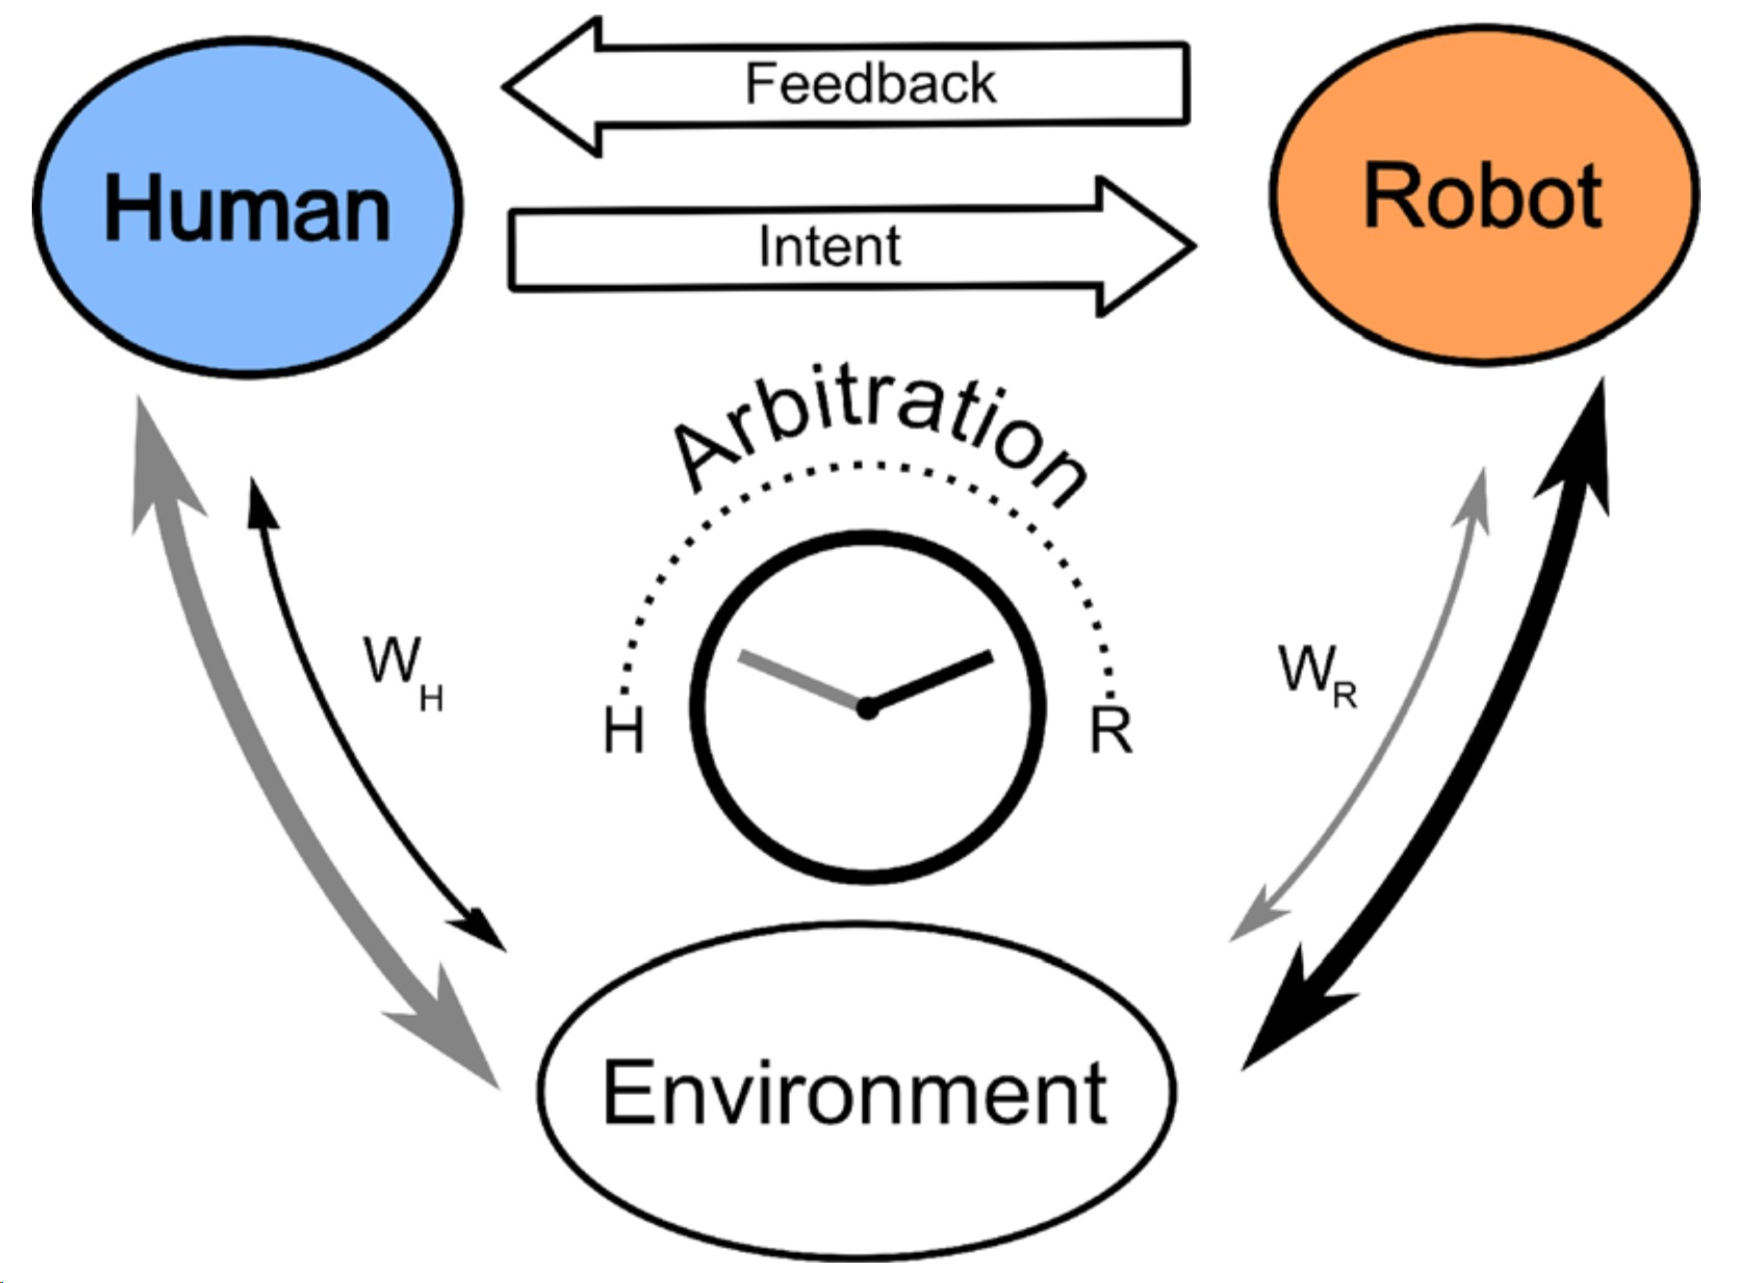
\includegraphics[width=0.8\linewidth]{figures/TradeStudy/figureb1.png}
%         \caption{Losey et al.'s proposed framework for human-robot interaction with the environment.}
%         % \label{figure:}
%     \end{center}
% \end{figure}
% 	Losey et al.'s 2018 review discusses the state of the art in the field of physical human-robot interaction, where human abilities are enhanced or supported by robotic aids, and discuss the human factors involved with shared task execution between the human and robot. They present a unified view of shared human-robot control in physical task execution, using case studies of applications in healthcare to demonstrate their framework. Their framework focuses on three distinct phases of decision making: detection, the task of understanding the human's intent; arbitration, the task of distributing control between the human and robot; and feedback, the task of presenting the result of the human's intent, which is often done through haptic devices. One ongoing field of research in physical human-robot interaction is that of dynamic changes in role arbitration using machine learning and artificial intelligence techniques. The authors note role arbitration should re-evaluated when trust changes, and further note "robotic performance has the largest and most identifiable influence on trust in HRI." As such, the real-time monitoring of performance metrics is an area of active research.

% Wang, Tian-Miao, Yong Tao, and Hui Liu. "Current Researches and Future Development Trend of Intelligent Robot: A Review." International Journal of Automation and Computing (2018): 1-22.
% 	In their 2018 review, Wang et al. discuss current research and future development trends of "intelligent" robots. They note several key and leading technologies in the field of robotics. They include key technologies such as human-robot collaboration technology, autonomous navigation technology under non-structured environments, multi-agent robot systems (swarms), and emotion recognition and interaction mechanism of robot oriented to harmonious human-robot cooperation. They also highlight innovative leading technologies such as brain computer interfaces, brain-like robot control and decision making (artificial intelligence and supervised/unsupervised learning techniques), material cross-innovation and applications of robot oriented to software structure (3D printed materials, soft grippers, flexible robots), and network decision mechanism of robot based on cloud computing and big data (IoT, SLAM). Their review further breaks down these technology areas into more specific, individual technologies and notes the current state of the art in each.
